\documentclass{beamer}
%\documentclass[handout]{beamer}
 \mode<presentation>{ 
 \usetheme{Antibes}%\usetheme{Warsaw}  
\setbeamercovered{invisible}
   %\usecolortheme{albatross} % for inverted color
% \usecolortheme{wolverine} % way too flashy!
    %\usefonttheme{structurebold}
    %\usetheme{Berkeley}
    % or ...    \setbeamercovered{transparent}
    % or whatever (possibly just delete it)
 
 } 
%\mode<handout>

 \frametitle{Traducció automàtica estadística}


\usepackage[spanish]{babel}
\usepackage[utf8]{inputenc}
\usepackage{times}
\usepackage{url}
\usepackage[T1]{fontenc}
\usepackage{alltt}
\usepackage[normalem]{ulem}
\newcommand{\empha}[1]{\emph{#1}}
\title[Traducción automática para la gente]{Traducción automática para la gente: no sólo para profesionales de la traducción}

\author[M.L.\ Forcada]{Mikel L.\ Forcada\inst{1,2}}

\institute[Universitat d'Alacant i Prompsit]{ 
\inst{1}Departament de Llenguatges i Sistemes Informàtics,\\
Universitat d'Alacant,  03071 Alacant \\[0.2cm]
\inst{2}Prompsit Language Engineering, S.L., \\ Edifici Quorum III, Av. Universitat s/n, 03202 Elx}


\date[Torrevieja 15/11/2017]{Torrevieja Científica: Jornadas de Tecnología Informática \\
Centro Cultural Virgen del Carmen, 
Torrevieja \\ 15 de noviembre de 2017}



%\newcommand{\curs}{Traducció Automàtica: Fonaments i Aplicacions}
%\newcommand{\llocidata}{Universitat d'Alacant, 2004}

\AtBeginSection[]
{
  \begin{frame}<beamer>{Outline}
    \tableofcontents[currentsection,currentsubsection]
  \end{frame}
}


\begin{document}

\frame{\maketitle}
% \begin{frame}
% \maketitle
% \titlepage
% \end{frame}


\begin{frame}<beamer>
\frametitle{Contents}
\tableofcontents
\end{frame}



\section{Las lenguas de Europa}

\begin{frame}
\frametitle{Las lenguas de Europa\ldots}

El multilingüismo forma parte del  \empha{alma} de la UE. 

\begin{itemize}
\item \textbf{24 lenguas oficiales en la UE (la ``lista de Lisboa''):}
% Move to three-letter
{\color{blue}
{\large bg}  {\large cs} {\normalsize da} {\huge de} {\large el} {\Huge en} {\Huge es} {\footnotesize et} {\normalsize fi} {\huge fr} {\tiny ga} {\normalsize hr} {\large hu} {\huge it} {\normalsize lt} {\footnotesize lv} {\scriptsize mt} {\Large nl} {\LARGE pl} {\huge pt} {\Large ro} {\normalsize sk} {\small sl} {\large sv}
}

\item \textbf{5 lenguas semi-oficiales de la UE:} 
{\color{blue}
{\normalsize ca}, {\normalsize cy}, {\small gl}, {\tiny gd}, {\scriptsize eu}.}

\item \textbf{Muchas lenguas no oficiales en paises de la UE:} 
{\color{blue}
{\tiny an}, {\small br}, {\tiny fo}, {\scriptsize fry}, {\scriptsize lb}, {\footnotesize oc}, \ldots
}

\item \textbf{Lenguas europeas que no son de la UE}
{\color{blue}
{\footnotesize is}, {\normalsize nb}, {\small nn}, {\large sr}, {\normalsize mk}, {\normalsize sq}, {\large uk}, {\normalsize be}, \ldots 
}

\item \textbf{Lenguas de la inmigración:} 
{\color{blue}
{\Huge ar}, {\Large ber}, {\Huge hi}, {\Huge ru}, {\Huge ur}, 
 {\Huge zh}.
}
\end{itemize}
(tamaño \(\simeq\) número total de hablantes en el mundo) 
\end{frame}

\begin{frame}
\frametitle{\ldots la Europa de las lenguas}
\begin{itemize}
\item Umberto Eco, 2003: \emph{La lingua dell'Europa è la traduzione}
\item Estudio \emph{The Europeans and their languages}, 2012:
\begin{quote}
El 46\% de la ciudadanía europea declara que sólo pueden mantener una conversación en su lengua materna.
\end{quote}
\item El multilingüismo de Europa se reproduce en España a pequeña escala:
\begin{itemize}
\item español, valenciano/catalán, gallego, occitano aranés, aragonés, asturiano\ldots
\end{itemize}
con varios niveles de protección legal.
\item Dependiendo de cual sea su lengua, las personas experimentan diferentes niveles de ciudadanía.
\end{itemize}

\end{frame}





%%%%%%%%%%%%%%%%%%%
\section{¿Qué es la traducción automàtica (TA)?}
\begin{frame}
\frametitle{¿Qué es la traducción automática (TA)? /1}

{
{La \empha{traducción}, \ldots }
\pause

{\ldots mediante un sistema informático \ldots}
\pause

{\ldots (ordenador(es) +
  programas) \ldots}
\pause

{\ldots de \empha{textos informatizados} en la \empha{lengua
    origen} (LO)\ldots}
\pause

{\ldots a \empha{textos informatizados} en la \empha{lengua meta}
  (LM).}

}
\end{frame}

%%%%%%%%%%%%%%%%%
\begin{frame}
  
\frametitle{¿Qué es la traducción automática (TA) /2?}

¿Ordenadores? 
\includegraphics[scale=0.02]{computer.png}

\includegraphics[scale=0.16]{laptop.png}\pause
\begin{itemize}
\item Bueno, también teléfonos móviles, tabletas, etc. 

\includegraphics[scale=0.02]{smartphone.png}
\includegraphics[scale=0.05]{tablet.png}
(que en el fondo son también ordenadores).\pause
\item Una buena parte del trabajo se hace en otros ordenadores: uno o
  más servidores conectados al nuestro por Internet (``la nube'').\\
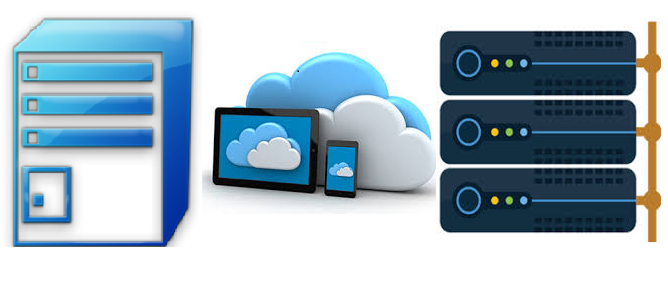
\includegraphics[scale=0.15]{cloud.png}
\end{itemize}
\end{frame}



\begin{frame}
  
\frametitle{¿Qué es la traducción automática (TA) /3?}

¿Programas?\pause
\begin{itemize}
\item También las \emph{aplicaciones} o \emph{apps} o los navegadores de Internet 
  como \emph{Chrome} o \emph{Firefox} son programas.\pause
\item Normalmente una parte del trabajo lo hace un programa en nuestro
  ordenador, móvil, tableta, y otra parte un programa en el servidor.\pause
\item Muchas veces ni siquiera lanzamos nosotros el sistema de traducción automática: se nos ofrece en navegadores y redes sociales.\pause
  \begin{itemize}
  \item De hecho, además de \emph{Google}, \emph{Facebook} desarrolla sus propios sistemas de TA.
  \end{itemize}\pause
\end{itemize}
\end{frame}


%%%%%%%%%%%%%%%%%%%

\begin{frame}
\frametitle{¿Què es la traducción automática (TA)? /4}

Esquemáticamente:

\begin{center}
\begin{tabular}{ccccc}
\framebox{\parbox{2.2cm}{\raggedright
\includegraphics[scale=0.07]{text.png}\\\textbf{Texto en lengua origen}}} & $\to$ & \framebox{\parbox{2.2cm}{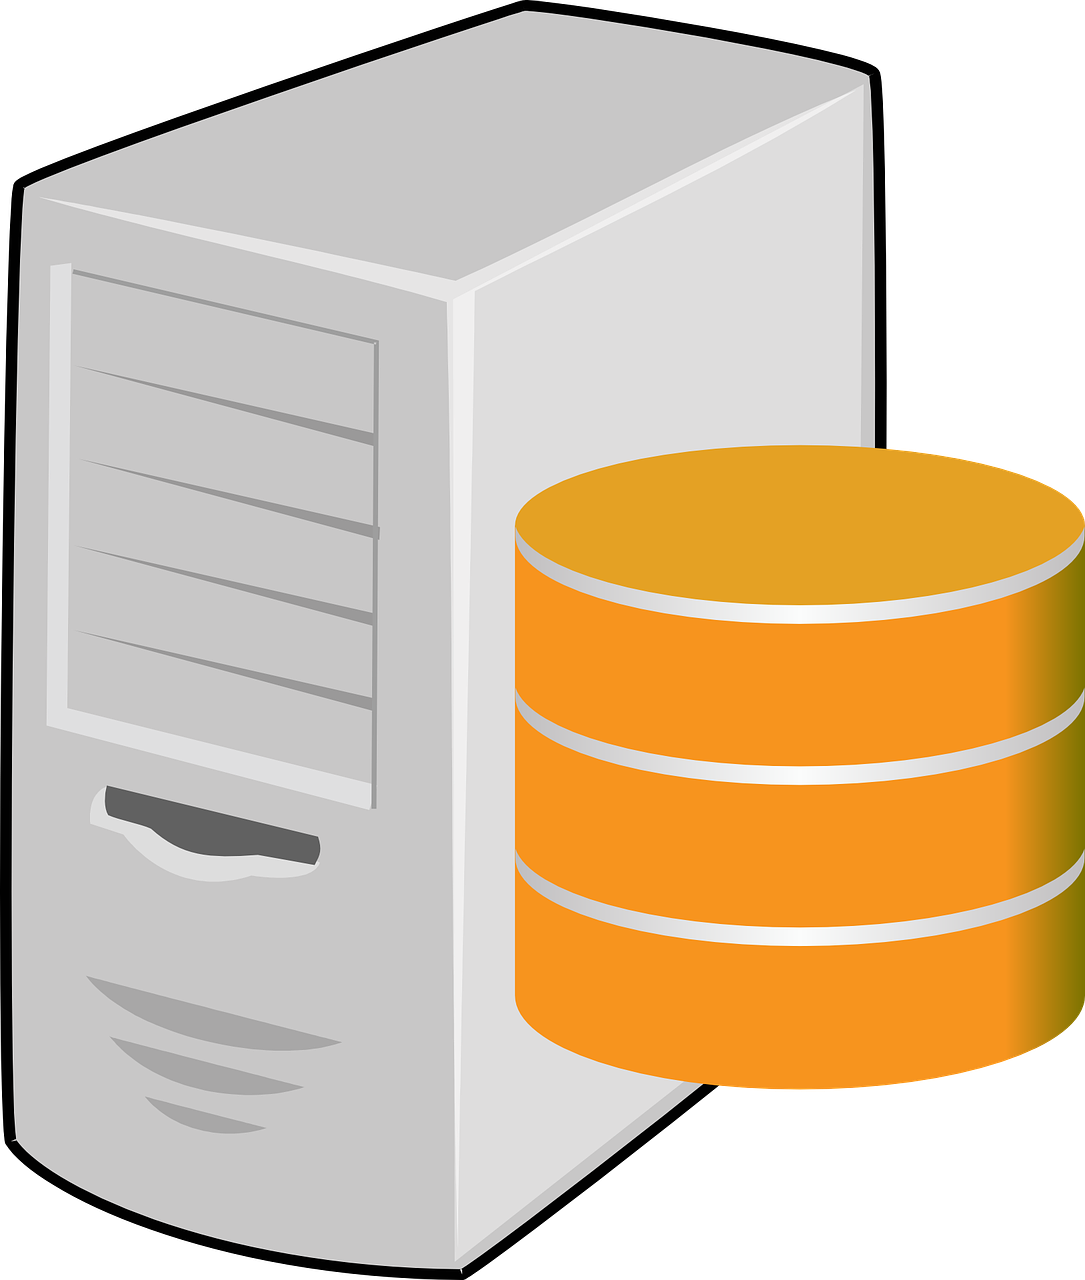
\includegraphics[scale=0.06]{computer-gearbox.png}\\Sistema de \\ traducción
    \\ automática}} & $\to$ & 
\framebox{\parbox{2.2cm}{\raggedright
\includegraphics[scale=0.07]{text.png}\\\textbf{Texto en lengua meta} (en bruto)}} \\ 
\end{tabular}
\end{center}


\end{frame}


\begin{frame}
\frametitle{¿Què es la traducción automática (TA)? /5}

La salida que producen los sistemas de traducción automática\ldots\pause
\begin{itemize}
\item \ldots no es como un producto profesional de traducción,\pause
\item \ldots normalmente no se puede publicar como está (pero a veces se hace), y\pause
\item \ldots muchas veces es la única traducción a la que se tiene acceso.\pause
\end{itemize}
¿Y cómo se usa?

\end{frame}

%%%%%%%%%%%%%%%%%%%



\section{Aplicaciones de la TA}


\begin{frame}
\frametitle{Aplicaciones de la TA /1}
Dos grandes grupos:\pause
\begin{itemize} 

\item\empha{\textbf{Diseminación:}} traducción \textbf{permanente}, idealmente
  \textbf{con pocos errores}, para su  \textbf{publicación}. P.ej.,
  producción de \textbf{borradores} para corregir
  (\textit{posteditar}).\pause
\begin{itemize}
\item Para \textbf{profesionales de la traducción}.\pause
\end{itemize}

\item\empha{\textbf{Asimilación:}} traducción \textbf{efímera}, idealmente
  \textbf{instantánea}, para la revisión o la \textbf{comprensión} de
  documentos en otra lengua que no conocemos. P.ej.,
  \empha{``navegación traduïda'' por Internet}, \textit{chat}
  multilingüe, etc.\pause
  \begin{itemize}
  \item ¡Para \textbf{el resto de la gente}!

  \end{itemize}

\end{itemize}

\end{frame}

\begin{frame}
\frametitle{Aplicaciones de la TA /2}

La \textbf{asimilación} es el uso más frecuente de la traducción automática.

Ya en 2012, Franz-Josef Och, \emph{científico distinguido} en el departamento de traducción automática de Google, decía:
\begin{quote}
En un dia cualquiera, traducimos aproximadamente tanto texto como el que contendrían un millón de libros. O, lo que es lo mismo, lo que todos los traductores profesionales traducen en un año, lo traduce nuestro sistema en aproximadamente un día.\footnote{\url{https://googleblog.blogspot.co.uk/2012/04/breaking-down-language-barriersix-years.html}}
\end{quote} 


\end{frame}

\begin{frame}
\frametitle{Aplicaciones de la TA /3}
Ejemplos de aplicaciones:\pause
\begin{itemize}
\item Leer en español la prensa extranjera.\pause
\begin{itemize}
\item De hecho, la BBC usa la TA para seguir qué dicen otros medios sobre los temas que forman parte de sus noticias.\pause
\item Ver que dicen en otro país cuando nuestro equipo juega allí.\pause
\end{itemize}
\item Aprender
\begin{itemize}
\item Por ejemplo, leer artículos de Wikipedia en otras lenguas\pause
\end{itemize}
\item Leer en español páginas escritas en otras lenguas oficiales de España\pause
\begin{itemize}
\item ¡Funciona mejor con el valenciano/catalán y el gallego que con el vasco!\pause
\end{itemize}
\item Aprender idiomas (por ejemplo, estudiando textos extranjeros).\pause
\item Tener amistades que hablan otros idiomas (usando la TA para comunicarnos).
\end{itemize}

\end{frame}

\begin{frame}
\frametitle{Aplicaciones de la TA/4}
¿Dónde encontramos traducción automática?\pause
\begin{itemize}
\item Aplicaciones para nuestro móvil: Google Translate, Apertium\ldots

\includegraphics[scale=0.09]{googletranslate.png}
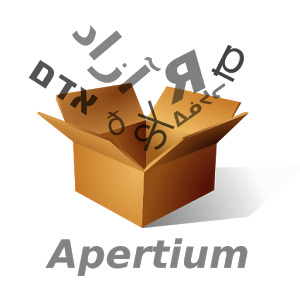
\includegraphics[scale=0.11]{apertium.png}\pause
\item Navegadores habilitados (como Chrome o Chromium) que incluyen traducción automática.\pause
\item Redes sociales (por ejemplo, Twitter ofrece traducciones automáticas de los tuits).\pause
\item Páginas web: \emph{Google Translate}, \emph{Bing Translator}, \emph{DeepL}, \emph{Lucy Software}, \emph{Apertium} etc.

\includegraphics[scale=0.09]{googletranslate.png}

\includegraphics[scale=0.1]{bing.png}

\includegraphics[scale=0.25]{deepl.png}

\includegraphics[scale=0.2]{lucy.png}
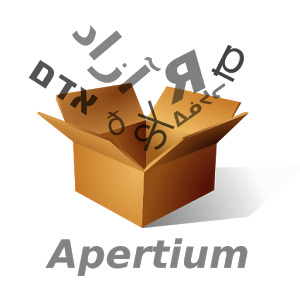
\includegraphics[scale=0.11]{apertium.png}
\pause
\end{itemize}
\end{frame}

%%%%%%%%%%%%%%%%%%%
\begin{frame}
  \frametitle{Asimilación: un texto en irlandés/1}

  \framebox{\parbox{\textwidth}{
  \empha{Is ar an Oileán Fada a bhí mé féin agus m’fhear céile ag fanacht
  nuair a rinne muid an turas sin. Dúradh linn fanacht cois farraige
  ag am díthrá agus thuirling an muireitleán anuas chun sinn a
  thabhairt ar bord. Bhí dream beag ar an turas mar níor thóg an
  t-eitleán sin thar deichniúr in am ar bith. Níl cur síos ar na
  radhairc a chonaic muid ar an aistear go dtí an mhórsceir.  Taobh
  istigh d’uair an chloig, bhí an mhórsceir féin bainte amach againn
  agus ba dhochreidte na radhairc a chonaic muid os ár gcomhair.}}}\pause
\begin{itemize}
\item El sistema de escritura del irlandés usa el mismo alfabeto del
  español (de hecho, no todas las letras), pero\ldots
\item ¿Alguien se anima a decir de qué va?

\end{itemize}
  \end{frame}
%%%%%%%%%%%%%%%%%%%
\begin{frame}
  \frametitle{Asimilación: traducción de Google Translate (2-nov-2017)}

  \framebox{\parbox{\textwidth}{

  \empha{Yo y mi esposo estábamos esperando Long Island cuando hicimos ese viaje. Nos dijeron que nos quedáramos por mar en el momento del engaño y aterrizamos en el avión para abordarnos. El viaje fue muy pequeño ya que el avión no tomó más de diez en ningún momento. No hay descripción de las escenas que vimos en el viaje al mayor. En una hora, habíamos llegado a nuestro propio pozo y las escenas que vimos fueron increíbles.}}}\pause
\begin{itemize}
\item ¿Y ahora, alguien puede decir de qué va?
\item ¿Hay algún lugar en el que nos hayamos atascado?
\end{itemize}

\end{frame}
%%%%%%%%%%%%%%%%%%%
\begin{frame}
  \frametitle{Asimilación: lo que quería decir (poco más o menos)}
  \framebox{\parbox{\textwidth}{
\empha{\textbf{Fue en Long Island donde mi esposo y yo} estábamos \textbf{hospedados} cuando hicimos ese viaje. Nos dijeron \textbf{que quedáramos a la orilla del} mar en el momento de \textbf{la bajamar, donde aterrizaría}  el \textbf{hidroavión} para \textbf{que lo abordáramos}. El \textbf{grupo era} muy pequeño ya que el avión no \textbf{podía llevar a} más de \textbf{diez personas en} ningún momento. No \textbf{se pueden describir} las escenas que vimos en el viaje al \textbf{arrecife}. En una hora, habíamos llegado \textbf{al propio arrecife} y las escenas que vimos fueron increíbles.}
}}
\pause
Errores extraños:
\begin{itemize}
\item ¿Por qué el \empha{hidroavión} se convierte en un \empha{avión} normal?
\item ¿\empha{arrecife}:  \empha{mayor} o \empha{pozo}?
\item ¿\empha{bajamar}: \empha{engaño}?
\end{itemize}

\end{frame}


%%%%%%%%%%%%%%%%%%%

\begin{frame}
\frametitle{Aplicaciones de la TA /5}

\empha{Postedición y preedición}: los professionales colaboran con el
  sistema de TA en aplicaciones de \textbf{diseminación}:
\begin{itemize}
\item\empha{Postedición:} corrección del texto traducido en bruto para hacerlo adecuado al propósito previsto (en seguida veremos un ejemplo).
\item Un paso más: \empha{preedición} o preparación del texto para evitar
  léxico o construcciones que dan problemas de traducción conocidos con un
  sistema de traducción automática determinado. 
  \begin{itemize}
  \item Interesa si el mateix mismo original se tiene que traducir a muchas lenguas meta (una preedición puede ahorrar más de una postedición).

  \end{itemize}
\end{itemize}

  Los profesionales deben conocer \empha{cómo funciona} el sistema de TA para usarlo de manera eficiente en sus tareas.

\end{frame}
%%%%%%%%%%%%%%%%%%%


%%%%%%%%%%%%%%%%%%%

\begin{frame}
  \frametitle{Ejemplo de postedición: texto original en portugués} 

  \framebox{\parbox{\textwidth}{
  \empha{Nova Iorque teve ontem uma noite de festa, após a aprovação
    durante a tarde (madrugada em Lisboa) pelo Senado estadual da lei
    que reconhece o direito ao casamento homossexual, por 33 votos
    contra 29, após anos de falhanço nesta câmara-alta.  O
    \underline{projecto} de lei tinha até aqui sido aprovado quatro
    vezes pela Assembleia do Estado, mas tinha sido sempre
    \textbf{rejeitada} pelo Senado de Nova Iorque, que agora se torna
    no sexto \textbf{estados} dos EUA a permitir o casamento entre
    pessoas do mesmo sexo.}}}

  \begin{itemize}
  \item El texto original tiene dos errores (en negrita).
  \end{itemize}

\end{frame}



\begin{frame}
  \frametitle{Traducción en bruto al español (apertium-pt-es)}

  \framebox{\parbox{\textwidth}{
  \empha{Nueva York tuvo ayer una noche de fiesta, después de la
    aprobación durante la tarde (madrugada en Lisboa) por Senado
    estadual de la ley que reconoce el derecho a la boda homosexual,
    por 33 votos contra 29, después de años de fracaso en esta
    @câmara-alta.  El @projecto de ley tenía hasta aquí sido aprobado
    cuatro veces por la @Assembleia del Estado, pero había sido
    siempre rechazada por Senado de Nueva York, que ahora se hace en
    el sexto estados de los EUA a permitir la boda entre personas del
    mismo sexo.}}}


  \begin{itemize}
  \item El sistema \emph{se ha atragantado} con algunas palabras que ha marcado con ``@''.
  \end{itemize}
\end{frame}

\begin{frame}
  \frametitle{Texto posteditado (postedición rápida)}

  \framebox{\parbox{\textwidth}{

  \empha{Nueva York tuvo ayer una noche de fiesta, después de la
    aprobación durante la tarde (madrugada en \textbf{Torrevieja}) por
    \textbf{el} Senado estadual de la ley que reconoce el derecho
    \textbf{al matrimonio} homosexual, por 33 votos contra 29, después
    de años de fracaso en esta \textbf{cámara alta}.  El
    \textbf{proyecto} de ley \textbf{había sido hasta hora} aprobado
    cuatro veces por la \textbf{Asamblea} del Estado, pero había sido
    siempre \textbf{rechazado} por \textbf{el} Senado de Nueva York, que ahora
    se \textbf{convierte} en el sexto \textbf{estado} de los
    \textbf{EEUU en} permitir \textbf{bodas} entre personas del mismo
    sexo.}}}

  \begin{itemize}
  \item Los cambios se indican en negritas.
  \item Algunos errores provienen de errores en el texto original.
  \end{itemize}
\end{frame}
%%%%%%%%%%%%%%%%%%%

\section{¿Cómo funciona la TA?}

\begin{frame}
  \frametitle{¿Cómo funciona la TA? /1}
Dos grandes tecnologías: \pause
\begin{itemize}
\item la \textbf{traducción automática basada en reglas (TABR)} \pause y
\item la \textbf{traducción automática basada en corpus (TABC)} \pause
\end{itemize}
Por supuesto hay tecnologías híbridas.
\end{frame}
%%%%%%

\begin{frame}
  \frametitle{¿Cómo funciona la TA? /2}

La \textbf{traducción automàtica basada en reglas (TABR)}
  \begin{itemize}
  \item Era la aproximación dominante en productos comerciales hasta hace
    unos doce años.\pause
  \item Personas expertas
    \begin{itemize}
    \item compilan diccionarios electrónicos,
    \item formulan reglas gramaticales y de traducción, y 
    \item escriben programas que los aplican al texto.
    \end{itemize}\pause
  \item Ejemplos en Internet: \empha{Lucy}, \empha{Apertium}.
  \end{itemize}
\end{frame}


\begin{frame}
  \frametitle{¿Cómo funciona la TA? /3}
La \textbf{traducción automática basada en corpus (TABC)}:
  \begin{itemize}
  \item Es actualmente la aproximación más pujante (el ''estado de la
    cuestión'').\pause
  \item Los sistemas \textbf{\emph{aprenden} a traducir} a partir de enormes
    corpus de texto bilingüe alineado oración a oración.\pause
  \item Lo que aprenden són complejos modelos estadísticos o
    ``neuronales''.
  \end{itemize}
\end{frame}


\begin{frame}
\frametitle{¿Cómo funciona la TA? /4}
El sistema no conoce las lenguas, simplemente busca correspondencias:
\begin{center}
  \begin{tabular}{l|l}
  \textbf{Lengua origen} & \textbf{Lengua meta} \\
  \hline
  an pifo & gur trafi \\
  an pifo onapi & gur manga trafi \\
  an saybe & gur suble \\
  \end{tabular}
\end{center}\pause
\begin{itemize}
\item ¿Qué podríamos deducir de estas traducciones?\pause
\item ¿Cómo traduciríamos ``an saybe onapi''? ¿Por qué?\pause
\item Un ordenador puede aprender diccionarios y reglas.
\end{itemize}
\end{frame}

\begin{frame}
\frametitle{¿Cómo funciona la TA? /5}

La \textbf{traducción automática estadística}:
\begin{itemize}
\item Aprende correspondencias entre fragmentos de oración y calcula probabilidades contando cuántas veces aparecen:
\begin{center}
  \begin{tabular}{l|l|r}
  \textbf{Fragmento inglés} & \textbf{Fragmento español} & Probabilidad \\
  \hline
  the  & la  & 17\% \\
  the  & el & 35\% \\
  the  & las & 22\% \\
  the  & los & 26\% \\
  the car & el coche & 85\% \\
  the house & la casa & 87\% \\
  large car & coche grande & 95\% \\
  a beautiful house & una casa preciosa & 78\% \\
  \ldots & \ldots & \ldots \\
  \end{tabular}
\end{center}

\end{itemize}
\end{frame}

\begin{frame}
  \frametitle{¿Cómo funciona la TA? /6}
  Después:
  \begin{itemize}
  \item Trocea la oracion original de todas las maneras posibles.\pause
  \item Busca las traducciones de los trozos.\pause
  \item Ensambla los trozos de todas las maneras posibles.\pause
    \begin{itemize}
    \item Vale, no todas: descarta muchas para ahorrar tiempo.\pause
    \end{itemize}
  \item Y usa 
    \begin{itemize}
    \item las probabilidades de traducción y\pause
    \item un modelo estadístico (¡otro!) de la lengua meta\pause
    \end{itemize}
   para elegir el montaje más verosímil como traducción.\footnote{Imagen tomada de Phillip Koehn (2010) \emph{Statistical Machine Translation}. Cambridge University Press}
  \end{itemize}
\begin{center}
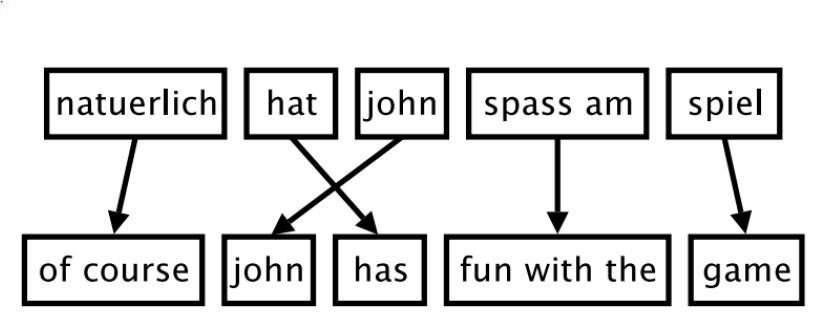
\includegraphics[scale=0.21]{phrasebasedexample.jpg}
\end{center}
\end{frame}

\begin{frame}
\frametitle{¿Cómo funciona la TA? /7}
\textbf{La traducción automática neuronal} (2013) (con precursores en 1997)\pause{}
 va montando la traducción
\begin{itemize}\pause
\item escogiendo una a una la palabra más probable que sigue a las anteriores: \footnote{Figura de \url{https://github.com/OpenNMT/}}\pause
  \begin{itemize}
  \item ``Mi \pause vuelo \pause se \pause retrasó\pause.''
  \end{itemize}
\item teniendo en cuenta la representación construida para la oración original
  \begin{itemize}
  \item \emph{My flight was delayed.}\pause
  \end{itemize}
\end{itemize}
\begin{center}
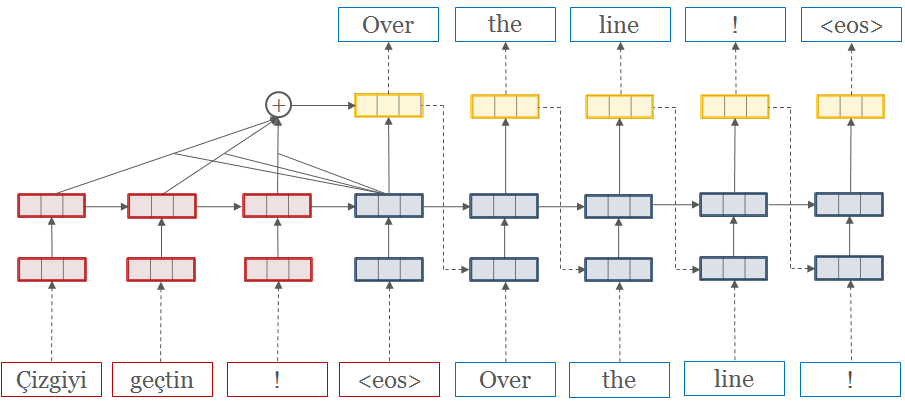
\includegraphics[scale=0.3]{nmt.png}
\end{center}

\end{frame}

\begin{frame}
\frametitle{¿Cómo funciona la TA? /8}
La traducción automática \textbf{neuronal}\pause
\begin{itemize}
\item Aprende a construir \textbf{representaciones internas}\pause
  \begin{itemize}
  \item de cada palabra de las lenguas origen y meta\pause
  \item de la oración original\pause
  \item de la traducción que va montando\pause
  \end{itemize}
\item Cada representación es un \textbf{patrón} formado por los valores de
  \emph{activación} de un grupo de \textbf{neuronas artificiales}\pause
  \begin{itemize}
  \item más o menos como cada posible imagen en una
    resonancia del cerebro\pause
  \item unas neuronas \textbf{activan} o \textbf{inhiben} a otras y así van construyendo las
    representaciones.
  \end{itemize}


\end{itemize}


\end{frame}

\section{Retos}
\begin{frame}
\frametitle{Retos /1}

La traducción automática se enfrenta con numerosos retos.\pause


Por ejemplo, las \textbf{oraciones} de un texto pueden ser
\textbf{ambiguas} (es decir, tener más de una interpretación):\pause

\begin{itemize}
\item porque sus palabras tengan más de una interpretación (ambigüedad
  \empha{léxica})\pause


\item porque la oración tenga más de una posible estructura  (ambigüedad \empha{estructural} o \empha{sintáctica})\pause

\item o incluso por las dos cosas a la vez.\pause
\end{itemize}
(Enseguida vemos unos ejemplos)
\end{frame}
%\textbf{[posar exemples ací?]}

\begin{frame}
\frametitle{Retos /2}
\begin{itemize}
\item Elegir la interpretación correcta no es trivial para un sistema
informático (que sólo tiene acceso al texto mismo).\pause
\begin{itemize}
\item Aunque recientemente se investiga en cómo usar  contexto: imágenes, perfiles personales, etc. (traducción automática multimodal).\pause
\end{itemize}

\item Las personas usamos nuestra experiencia, nuestras expectativas y nuestro conocimiento del mundo para elegir.

\end{itemize}


%\textbf{[posar exemples ací?]}

\end{frame} 

\begin{frame}
  \frametitle{Retos /3}
  Ambigüedades léxicas:
  \begin{itemize}
  \item \emph{--- Le vendo un coche. ---Y yo ¿para qué quiero un coche vendado?}\pause
    \begin{itemize}
    \item \emph{vendo}: ¿\emph{vender} o \emph{vendar}?
    \end{itemize}\pause
  \item \emph{Trabaja en el estudio que le encargaron.}\pause
    \begin{itemize}
    \item \emph{estudio}: ¿\emph{informe}, \emph{taller}, \emph{pequeño apartamento}\ldots?
    \end{itemize}\pause
  \end{itemize}
\end{frame}


\begin{frame}
  \frametitle{Retos /4}
  Ambigüedades estructurales:
  \begin{itemize}
  \item \emph{Aprendió a afeitarse en treinta segundos.}\pause
    \begin{itemize}
    \item ¿Tiempo de afeitado o tiempo de aprendizaje?\pause
    \item \emph{\framebox{aprendió a} \framebox{afeitarse \framebox{en treinta segundos}}} \pause
    \item \emph{\framebox{\framebox{aprendió a} \framebox{afeitarse}} \framebox{en treinta segundos}} 
    \end{itemize}
  \end{itemize}
\end{frame}

\begin{frame}
  \frametitle{Retos /5}
  Ambigüedades estructurales:
  \begin{itemize}
  \item \emph{Trajo noticias de Grecia}\pause
    \begin{itemize}
    \item ¿Procedentes de Grecia o sobre Grecia?\pause
    \item \emph{\framebox{Trajo}\framebox{noticias \framebox{de Grecia}}}\pause
    \item \emph{\framebox{Trajo \framebox{noticias}} \framebox{de Grecia}}\pause
    \end{itemize}
  \item \emph{Se vende piso con ascensor de 90 m$^2$}\pause
    \begin{itemize}
    \item ¡Vaya pedazo de ascensor!
    \end{itemize}
  \end{itemize}
\end{frame}

\begin{frame}
\frametitle{Retos /6}
La ambigüedad no es el único reto. La tarea no es fácil.\pause

Los sistemas de traducción automática a veces tienen que \textbf{reordenar} completamente las palabras de la oración (cuando las lenguas tienen estructuras muy diferentes):\pause
\begin{center}
  \emph{Donostiako\ $^1$ gizon\ $^2$ haundi\ $^3$ harek\ $^4$ zekarren\ $^5$ automobila\ $^6$} \\ \pause
  $\downarrow$
  \\
  \emph{[El coche]\ $^6$ [que traía]\ $^5$ aquel\ $^4$ hombre\ $^2$ grande\ $^3$ [de San Sebastián]\ $^1$} \\[1cm]\pause
 1--2--3--4--5--6 $\to$ 6--5--4--2--3--1 ! 
\end{center}
\end{frame}

\section{Comentarios finales}

\begin{frame}
\frametitle{Para ir acabando\ldots}

Espero\ldots\pause
\begin{itemize}
\item \ldots que hayan aprendido un poquito más sobre la traducción automática como tecnología.\pause
\item \ldots que se animen a usarla más en su vida cotidiana para saltarse las barreras lingüísticas.\pause
\item \ldots ¡que tengan muchas preguntas para mí!\pause
\end{itemize}
¡Muchas gracias!

\end{frame}

\end{document}


%%%%%%%%%%%%%%%%%%%

%%%%%%%%%%%%%%%%%%%%%%%%%%%%%%%%%%%%%%%%%%%%%

\begin{frame}
  \frametitle{ Com funciona la TA? /19} 
  
  \textbf{Per tant, tant si usem regles com estadística...}

  \begin{itemize}
  \item \empha{Podem esperar}, en el millor cas, que un bon sistema de TA 
    \begin{itemize}
    \item ens allibere de la
      part més \empha{mecànica} (mecanitzable) de la tasca de traducció i
    \item ens permeta concentrar-nos en la part més \empha{creativa} (per exemple, durant la postedició).
    \end{itemize}


  \item Però \empha{no hem d'esperar} ---per bo que siga--- que 
    \begin{itemize}
    \item comprenga
      el text, 
    \item resolga les ambigüitats sempre correctament i 
    \item produïsca
      textos en una variant genuïna de la llengua meta.
    \end{itemize}
  \end{itemize}

\end{frame}



%%%%%%%%%%%%%%%%%%%%%%%%%%%%%%%%%%%%%%%%%%%%%
\section{Per què és difícil la TA?}
\begin{frame}
  \frametitle{ Per què és difícil la TA? /1} 

   {
  {Els quatre problemes de la traducció automàtica (Arnold 2003):}
  \begin{enumerate}
   {\item El problema de l'anàlisi}
   {\item El problema de la síntesi}
   {\item El problema de la transferència}
   {\item El problema de la descripció}
  \end{enumerate}
  }

  
\end{frame}

\begin{frame}
  \frametitle{ Per què és difícil la TA? /2} 
  
  \textbf{El problema de l'anàlisi:} La forma no determina completament el
  contingut (la \empha{interpretació}). També s'anomena \empha{ambigüitat}. 
  Com hem vist, l'ambigüitat pot ser:
  \begin{itemize}
  \item \textbf{Estructural} o sintàctica:
  \begin{itemize}
  \item \empha{Portaven notícies de Grècia} (tema o procedència?)
  \item \empha{Ha venut les taronges que ha
  comprat a Joan} (Joan ven o compra?)
  \item \empha{La direcció s'oposa a implantar mesures per evitar la crisi} (realment vol evitar la crisi?)
  \end{itemize}
  \item \textbf{Lèxica} 
    \begin{itemize}
  \item \empha{Treballa en l'estudi que li han encarregat} (prepara un document
  o dissenya un taller d'artista?)
  \item \empha{El gat és sota el cotxe} (felí o màquina d'alçar cotxes?)
    \end{itemize}
  \item O fins i tot \textbf{mixta}:
    \begin{itemize}
    \item Les gallines han destrossat el sembrat però no les mates (destrucció parcial? càstig severíssim?)
    \end{itemize}
  \end{itemize}
\end{frame}


%%%%%%%%%%%%%%%%%%%%%%%%%%%%%%%%%%%%%%%%%%%%%%%%%%%%%%%%%%%%%%%%%%%%%
\begin{frame}
  \frametitle{ Per què és difícil la TA? /3} 
  
  \textbf{El problema de la síntesi} (o de la generació): El contingut
  no determina completament la forma (hi ha més d'una manera de dir el
  mateix en qualsevol llengua, però només una és \empha{genuïna} o la
  més adequada per al propòsit previst):
  \begin{itemize}
  \item \empha{Quina hora és?}
  \item \empha{Com és de tard?} (\texttt{de}: \empha{Wie spät ist es?})
  \item \empha{Quines hores són?} (\texttt{pt}: \empha{Que horas s\~{a}o?})
  \item \empha{Quantes del rellotge són?} (\texttt{de}: \empha{Wieviel Uhr ist es?})
  \end{itemize}

  Els \empha{expedients} s'\empha{obrin} o s'\empha{inicien}?

  Les sessions es \empha{clouen}, es \empha{tanquen}, es \empha{rematen} o \empha{s'alcen}?

\end{frame}

%%%%%%%%%%%%%%%%%%%%%%%%%%%%%%%%%%%%%%%%%%%%%%%%%%%%%%%%%%%%%%%%%%%%%
\begin{frame}
  \frametitle{ Per què és difícil la TA? /4} 
  
  \textbf{El problema de la transferència:} Les llengües divergeixen. És a
  dir, hi ha diferències irreductibles en la manera en que el mateix contingut
  s'expressa en llengües diferents:
  \begin{itemize}\itemsep 0ex
  \item \texttt{ca:} \empha{M'agrada nadar} (\empha{M'} objecte, \empha{agrada},
    verb, \empha{nadar} subjecte)
  \item \texttt{en:} \empha{I like swimming} (\empha{I} subjecte, \empha{like}
  verb, 
  \empha{swimming} objecte)
  \item \texttt{de:} \empha{Ich schwimme gern} (\empha{Ich} subjecte,
  \empha{schwimme}, verb,  \empha{gern}, adverbi)
  \end{itemize}
  Totes volen dir \texttt{produir\_plaer(agent=nadar(agent=jo),destinatari=jo)}
\end{frame}


%%%%%%%%%%%%%%%%%%%%%%%%%%%%%%%%%%%%%%%%%%%%%%%%%%%%%%%%%%%%%%%%%%%%%
\begin{frame}
  \frametitle{ Per què és difícil la TA? /5} 
  
  \textbf{El problema de la descripció} (represa): construir un sistema de
  traducció automàtica comporta la gestió d'una gran quantitat de coneixement,
  que s'ha d'elicitar, arreplegar, descriure, i representar en una forma útil i
  computable:
  \begin{itemize}
  \item que el femení d'\empha{orfe} és \empha{òrfena} i el plural de \empha{llapis} és \empha{llapis}
  \item que la traducció de \empha{coixí} (masc.) és \empha{almohada} (fem.)
  \item que la forma que pren \empha{en}  davant de topònim és \empha{a}
  \item que \empha{Dénia}, \empha{Olot}\ldots són topònims (i \empha{Toni} no)
  \item que cal llevar la preposició \empha{de} davant \empha{que} en català
  \item que en una seqüència \textbf{det--subst--adj}, si el substantiu canvia de gènere en traduir, cal canviar el del determinant i l'adjectiu però només si l'adjectiu concordava ja amb el substantiu\ldots
  \end{itemize}
Els sistemes estadístics tenen altres dificultats (arreplegar corpus representatius, \emph{netejar-los}, alinear-los\ldots).

\end{frame}

%%%%%%%%%%%%%%%%%%%%%%%%%%%%%%%%%%%%%%%%%%%%%%%%%%%%%%%%%%%%%%%%%%%%%


\section{Avaluació de la TA}

\begin{frame}
  \frametitle{Avaluació de la traducció automàtica /1}

  \begin{itemize}
  \item   L'avaluació de la TA és encara un tema obert i controvertit per als
  especialistes:
  \begin{itemize}
  \item Com que l'avaluació humana és molt costosa (com veurem) hi ha
     mesures d'avaluació automàtica que comparen l'eixida
    del sistema amb un o més textos de referència.
  \item La capacitat d'aquestes mesures per a predir la utilitat de la
    TA en aplicacions concretes és encara molt limitada.
  \end{itemize}
  \item   Al mateix temps, és un tema sobre el qual molta gent inexperta
  s'aventura a donar opinions, normalment excessivament optimistes o
  excessivament pessimistes.
  \item   En general se sol oblidar que cal avaluar pensant en un \textbf{propòsit}.
  \item   Imaginem-nos una aplicació concreta i veurem per què no és gens fàcil.
  \end{itemize}






\end{frame}


\begin{frame}
  \frametitle{ Avaluació de la traducció automàtica /2}
{
{Volem avaluar \empha{l'adopció} d'un sistema de traducció
  automàtica per a la \empha{disseminació} (publicació).}
\begin{itemize}
\item Les traduccions en brut s'hauran de \empha{posteditar} (corregir): com
  menys correccions, més \empha{qualitat}: millor.
\item D'acord: com ho avaluem?
\end{itemize}


}
\end{frame}
%%%%%%%%%%%%%%%%%%%%%%%%%%%%%%%%%%%%%%%%%%%%%%%%%%%
%%%%%%%%%%%%%%%%%%%%%%%%%%%%%%%%%%%%%%%%%%%%%%%%%%%%%%%%%%%%%%%%%%%%%
\begin{frame}
  \frametitle{ Avaluació de la traducció automàtica /3}
{
{Per avaluar la \empha{qualitat}, cal:}
\begin{itemize}\itemsep 0ex
{\item elegir una mostra suficient de textos representatius,}
{\item traduir-la automàticament,}
{\item i comptar la quantitat de correcció \empha{mínima} necessària per
  a fer que la traducció siga \empha{adequada al propòsit previst}.}
\end{itemize}
{Sembla senzill, però...}


}
\end{frame}
%%%%%%%%%%%%%%%%%%%%%%%%%%%%%%%%%%%%%%%%%%%%%%%%%%%%%%%%%%%%%%%%%%%%%
\begin{frame}
  \frametitle{ Avaluació de la traducció automàtica /4}
{
{...no ho és gens!}
\begin{itemize}\itemsep 0ex
{\item és difícil elegir prou text representatiu per endavant;}
{\item la noció d'\empha{adequació} és de vegades difícil d'especificar:}
{\item és difícil fer el \empha{mínim} de correccions (cal buscar
  traduccions adequades que se n'obtinguen amb poques correccions);}
{\item tot el procés és molt costós (temps de correcció).}
\end{itemize}

}
\end{frame}
%%%%%%%%%%%%%%%%%%%%%%%%%%%%%%%%%%%%%%%%%%%%%%%%%%%
%%%%%%%%%%%%%%%%%%%%%%%%%%%%%%%%%%%%%%%%%%%%%%%%%%%%%%%%%%%%%%%%%%%%%
\begin{frame}
  \frametitle{ Avaluació de la traducció automàtica /5}
{
{Però la qualitat dels textos traduïts en brut no ho és tot!}

{Fem un \textbf{pressupost}: si adoptem la traducció automàtica,}

{d'una banda, ens estalviem els costos de traducció humana,}

{però tenim despeses noves:}

\begin{itemize}\itemsep 0ex
{\item despeses de \empha{funcionament} i}
{\item despeses de \empha{formació} (s'ha d'aprendre a usar una nova
  tecnologia)} 
\end{itemize}

}
\end{frame}
%%%%%%%%%%%%%%%%%%%%%%%%%%%%%%%%%%%%%%%%%%%%%%%%%%%
%%%%%%%%%%%%%%%%%%%%%%%%%%%%%%%%%%%%%%%%%%%%%%%%%%%%%%%%%%%%%%%%%%%%%
\begin{frame}
  \frametitle{ Avaluació de la traducció automàtica /6}
{
{Despeses de funcionament:}
\begin{itemize}\itemsep 0ex
  {\item \textbf{Cost del sistema de TA} (cost efectiu per mot):
    amortització (sistema en propietat), cost per mot (sistema llogat), servei
    tècnic i manteniment, costos de migració (adaptació de programes,
    adquisició de sistemes), i (no oblidem) el cost d'avaluació!}
  {\item \textbf{Cost de preedició i preparació:} potser cal preparar i 
    \emph{preeditar} els textos i això ho ha de fer algú, cobrant.}   {\item
      \textbf{Cost de postedició}: depén de la \empha{qualitat}; pot baixar amb
      la formació; depén de com paguem als posteditors (per mot, per temps),
      etc.}
\end{itemize}

}
\end{frame}
%%%%%%%%%%%%%%%%%%%%%%%%%%%%%%%%%%%%%%%%%%%%%%%%%%%%%%%%%%%%%%%%%%%%%
%%%%%%%%%%%%%%%%%%%%%%%%%%%%%%%%%%%%%%%%%%%%%%%%%%%%%%%%%%%%%%%%%%%%%
\begin{frame}
  \frametitle{ Avaluació de la traducció automàtica /7}
{
{Despeses de formació:}
\begin{itemize}\itemsep 0ex
  {\item \textbf{Formació en ús del programa de TA}: ús pròpiament dit,
    configuració i manteniment; ús de nou programari associat.}  
  
  {\item \textbf{Formació en postedició:}}
    \begin{itemize}\itemsep 0ex
    {\item coneixement del programa de TA
    (errors típics);}
    {\item tècniques de correcció, ús avançat del processador de textos,
    macroinstruccions, substitució de patrons, etc.}
    \end{itemize}
\end{itemize}
}

\end{frame}
%%%%%%%%%%%%%%%%%%%%%%%%%%%%%%%%%%%%%%%%%%%%%%%%%%%%%%%%%%%%%%%%%%%%%
\begin{frame}
  \frametitle{ Avaluació de la traducció automàtica /8}

{
  \begin{itemize}
  \item {I potser ens hem deixat encara alguna cosa!}
\pause

\item {Avaluar la traducció automàtica no és gens fàcil.}
\pause

\item {La lliçò? Desconfieu de les primeres impressions.}
  \end{itemize}

}
\end{frame}
%%%%%%%%%%%%%%%%%%%%%%%%%%%%%%%%%%%%%%%%%%%%%%%%%%%

\section{TA per al català}
\begin{frame}
  \frametitle{Traducció automàtica per al català/1}
%  \textbf{[un recompte del que hi ha]}
Hi ha bastants sistemes de TA per al català:
\begin{itemize}
\item \textbf{SALT} (v. 4.0), de la Generalitat Valenciana
  (\Pair{es}{ca}): instal·lable en Linux, Windows i Mac i accessible
  en línia (p.ex. \empha{Las Provincias}): gratuït (no lliure), gran
  cobertura lèxica, concebut per aprendre valencià.
  \begin{itemize}
  \item \url{http://www.edu.gva.es/polin/val/salt/apolin_salt.htm}
  \end{itemize}
\item \textbf{interNOSTRUM.com}, CAM/Universitat d'Alacant (\Pair{es}{ca}): en línia, molt usat en Internet, però ja no es manté.
  \begin{itemize}
  \item \url{http://www.internostrum.com}
  \end{itemize}
\end{itemize}
\end{frame}

\begin{frame}
  \frametitle{Traducció automàtica per al català/2}

Més sistemes:
\begin{itemize}
\item \textbf{Apertium.org} (\Pair{es}{ca}, \Pair{en}{ca}, \Pair{fr}{ca}, \Pair{pt}{ca}, \Pair{ca}{oc},  \pair{ca}{eo}): hereu d'\empha{interNOSTRUM.com}, en línia i descarregable, lliure/de codi font obert (l'explicaré més avall).
  \begin{itemize}
  \item \url{http://www.apertium.org}
  \end{itemize}
\item \textbf{Lucy Software} (\Pair{es}{ca}, \Pair{en}{ca}, \Pair{fr}{ca}, \Pair{ca}{de}, \pair{ca}{oc}): comercial, es pot provar en línia (abans \empha{Incyta}, \empha{Comprendium}, \empha{Translendium}\ldots).
  \begin{itemize}
  \item \url{http://www.lucysoftware.com/catala/inici/}
  \end{itemize}
\item \textbf{Automatic Trans} (\Pair{es}{ca}, \Pair{eu}{ca}, \Pair{gl}{ca}, \Pair{pt}{ca}): comercial, grans clients, relacionat amb l'usat cada dia a \empha{El Periódico de Catalunya}.
  \begin{itemize}
  \item \url{http://www.cat.automatictrans.es/}
  \end{itemize}
\end{itemize}

\end{frame}
\begin{frame}
  \frametitle{Traducció automàtica per al català/2}

Més sistemes:
\begin{itemize}
\item \textbf{SisHiTra} (\Pair{es}{ca}), UPV: ``Sistema Híbrid de Traducció'' que combina regles lingüístiques amb models estadístics, resultats molt interessants.
  \begin{itemize}
  \item \url{http://sishitra.iti.upv.es/}
  \end{itemize}
\item \textbf{Google Translate} (de \texttt{ca} a més de 50 llengües): sistema estadístic de la companyia Google.
  \begin{itemize}
  \item \url{http://translate.google.com}
  \end{itemize}
\item \textbf{Bing Translator} (de \texttt{ca} a més de 20 llengües): sistema estadístic de la companyia Microsoft.
  \begin{itemize}
  \item \url{http://www.microsofttranslator.com/}
  \end{itemize}
\end{itemize}

\end{frame}

\begin{frame}
  \frametitle{Traducció automàtica per al català /4}

\textbf{Quin és el millor sistema?}

Consell: abans de prendre una decisió, proveu-los tots, tenint en compte
\begin{itemize}
\item la qualitat de la traducció per al vostre propòsit
\item el preu
\item possibles limitacions a la grandària o el format dels textos
\item si preserven o no el format del text, etc.
\end{itemize}
Recordeu el que hem discutit abans quant a l'avaluació!
\end{frame}


\section[Traducció automàtica lliure]{TA lliure o de codi font obert}


\begin{frame}
\frametitle{Què és el programari lliure o de codi font obert?}
El programari és \empha{lliure} (Free Software Foundation, \url{www.fsf.org}) quan:
\begin{itemize}
\item[0] hom es lliure d'usar el programa per a qualsevol propòsit
\item[1] hom pot estudiar com funciona el programa, i adaptar-lo a les seues necessitats
\item[2] hom pot distribuir còpies i ajudar així el veí
\item[3] hom pot millorar el programa i fer públiques les millores als altres, de manera que tota la comunitat se'n beneficie
\end{itemize}
Perquè les condicions 1 i 3 es complisquen, s'ha de tenir accés al codi font (tal com l'ha escrit el programador). Per això se'n diu també \empha{programari de codi font obert} (Open Source Initiative, \url{www.opensource.org}).
\end{frame}

%\subsection*{Programari de traducció automàtica: obert o tancat?}

\begin{frame}
\frametitle{Peculiaritats del programari de traducció automàtica}
\begin{itemize}
\item La traducció automàtica (TA) és especial: depén fortament de l'existència de dades. Hi ha tres components en qualsevol sistema de TA:\footnote{TA ``basada en regles''; la TA ``basada en corpus'' té requisits anàlegs}
  \begin{itemize} 
  \item El \empha{motor} (el programa pròpiament dit)
  \item Les \empha{dades lingüístiques} (diccionaris, regles)
  \item Les \empha{eines} necessàries per a mantenir aquestes dades i convertir-les al format usat pel \empha{motor}
  \end{itemize}
\end{itemize}


\end{frame}

\begin{frame}
\frametitle{La traducció automàtica comercial, normalment de codi font tancat}
  \begin{itemize}
  \item Els sistemes comercials usen tecnologies \empha{privatives} o
    \empha{de propietat} (\empha{proprietary}) que no es revelen (el fabricant
    les percep com un avantatge competitiu fonamental)
  \item Típicament, només s'hi permet la modificació parcial (\empha{personalització}) de les dades lingüístiques.
  \item Que un sistema es puga usar a Internet no vol dir que siga lliure o de codi font obert (versions de prova, sistemes no comercials).
  \end{itemize}
\end{frame}

\begin{frame}
\frametitle{Traducció automàtica lliure o de codi font obert}
Perquè la TA siga lliure o de codi font obert, tant   
\begin{itemize}
\item el motor, 
\item les dades, 
\item com les ferramentes 
\end{itemize}
han de ser lliures o de codi font obert.
\end{frame}

\begin{frame}
\frametitle{Avantatges de la traducció automàtica lliure o de codi font obert}
\begin{itemize}
\item L'ús de sistemes de TA lliures o de codi font obert té
  avantatges específics sobre els sistemes comercials de codi font
  tancat.  Destaquem-ne dos:
 \begin{itemize}
 \item \empha{Augmenta la perícia} (\empha{expertise}, coneixement) de
   les comunitats lingüístiques implicades i \empha{els recursos
     lingüístics} disponibles per a elles (fixació, codificació i
   aplicació del coneixement), i els dissemina molt eficientment.
 \item \empha{Augmenta la independència} respecte d'un proveïdor
   comercial de traducció automàtica tancada (o d'altres tecnologies
   lingüístiques).
 \end{itemize}
\end{itemize}
\end{frame}



\begin{frame}
  \frametitle{Reptes de la traducció automàtica lliure o de codi font
    obert} Per a poder gaudir d'aquests avantatges, les comunitats
  lingüístiques implicades en la creació d'un nou sistema de TA han de
  fer front a reptes com :
  \begin{itemize}
  \item La neutralització d'actituds \empha{tecnofòbiques} (!)
  \item L'organització del desenvolupament comunitari
  \item L'\empha{elicitació} del coneixement lingüístic
  \item L'estandardització i documentació dels formats de les dades lingüístiques
  \item L'assoliment de la modularitat en  programes i dades.
  \end{itemize}

\end{frame}




\section{Apertium: un sistema de TA lliure/de codi font obert}

%\subsection*{Antecedents i fonaments}
\begin{frame}
 \frametitle{Antecedents} 

 Apertium està basat en les tecnologies creades pel grup Transducens
 de la Universitat d'Alacant durant el desenvolupament de dos sistemes
 existents:
 
\begin{itemize}
 
\item \textbf{interNOSTRUM} (\texttt{interNOSTRUM.com},
  \texttt{es}\(\leftrightarrow\)\texttt{ca}%\footnote{\scriptsize{La llengua amb codi ISO-639 \texttt{ca}, parlada a Xàtiva, Palma, Olot, Perpinyà\ldots, és coneguda com a \empha{català}, \empha{valencià}, \empha{mallorquí}, etc. i la immensa majoria dels qui l'escriuen bé usen bàsicament el mateix estàndard.}})
 
\item \textbf{Tradutor Universia} (\texttt{tradutor.universia.net},
  \texttt{es}\(\leftrightarrow\)\texttt{pt})
 
\end{itemize}

Aquestes tecnologies, inicialment dissenyades per a parells de
llengües estretament emparentades (com les romàniques!), han estat
esteses per a tractar parells de llengües més allunyats.

\end{frame}

%\subsection*{Fonaments}

\begin{frame}
\frametitle{Fonaments /1}

Per a generar traduccions que siguen: 

\begin{itemize}

\item raonablement intel·ligibles i
\item fàcils de corregir (posteditar)
\end{itemize}
entre llengües estretament emparentades com l'espanyol (\texttt{es}) i
el català (\texttt{ca}) o el portugués (\texttt{pt}), etc., només cal
millorar la traducció \empha{mot per mot} amb algunes operacions.

\end{frame}

\begin{frame}
\frametitle{Fonaments /2}

Millores sobre la traducció mot per mot: 
\begin{itemize}
\item processament lèxic robust (incloent-hi unitats lèxiques multi-mot)
  \begin{center}
    (es) \textit{echar de menos} \(\to\) (ca) \sout{\textit{tirar de menys}} \textit{trobar a faltar}
  \end{center}
\item desambiguació lèxica categorial (\empha{part-of-speech tagging})
  \begin{center}
    (es) \textit{amigas como ella} \(\to\) (ca) \textit{amigues \sout{menge} \textbf{com} ella} 
  \end{center}
\item processament estructural local basat en regles simples i ben formulades per a transformacions estructurals freqüents (reordenació, concordança):
  \begin{center}
    (es) \textit{un valle seco} \(\to\) (ca) \textit{\sout{un} \textbf{una} vall \sout{sec} \textbf{seca}}
  \end{center}
\end{itemize}

\end{frame}

\begin{frame}
  \frametitle{Fonaments /3}
Per a parells de llengües més difícils, no tan 
relacionats: 
\begin{itemize}
\item Hauria de ser possible estendre aquest model senzill.
\item Hauria de ser possible generalitzar-ne els conceptes de manera que la complexitat es mantinga tan baixa com siga possible.
\end{itemize}
\end{frame}


\begin{frame}
  \frametitle{Fonaments /4}
  
\begin{itemize}
  
\item Hauria de ser possible generar un sistema complet de traducció
  automàtica a partir de dades lingüístiques (diccionaris monolingües
  i bilingües, regles gramaticals), especificades de manera
  \textbf{declarativa}.
\item Aquestes dades: 
\begin{itemize}
\item regles (independents de la llengua) per a tractar formats de text
\item especificació del desambiguador lèxic categorial
\item diccionaris morfològics i bilingües i diccionaris de regles de transformació ortogràfica
\item regles de transferència estructural
\end{itemize}
haurien d'estar en un format interoperable  $\Rightarrow$ \textbf{XML}.
  
\end{itemize}

\end{frame}
\begin{frame}
  \frametitle{Fonaments /5}
  
\begin{itemize}
  
\item Hauria de ser possible tenir un motor de traducció únic (independent de la llengua) que llegiria dades específiques per a cada parell de llengües
  (``separació d'algorismes i dades'').
\item Les dades lingüístiques del parell de llengües haurien de ser preprocessades de manera que el sistema siga ràpid ($>$10,000 mots per segon) i compacte; per exemple, les transformacions lèxiques es farien amb transductors d'estats finits
  (TEFs).
\end{itemize}

\end{frame}
\begin{frame}
  \frametitle{Fonaments /6}
  
  Raons per al desenvolupament d'Apertium com a programari lliure o de codi font obert:
\begin{itemize}
\item Donar a tothom accés lliure i il·limitat a les millors tecnologies possibles de traducció automàtica.
\item Establir una plataforma modular, documentada i oberta per a la traducció automàtica de transferència superficial i per a altres tasques de processament automàtic de la llengua.
\item Afavorir l'intercanvi i la reutilització de les dades lingüístiques existents.
\item Facilitar la integració amb altres tecnologies lliures o de codi font obert.
\end{itemize}

\end{frame}
\begin{frame}
  \frametitle{Fonaments /7}
  
  Més raons per al desenvolupament d'Apertium com a programari lliure
  o de codi font obert:

\begin{itemize}
\item Beneficiar-se del desenvolupament col·laboratiu 
  \begin{itemize}
  \item del motor de traducció i de les eines
  \item de dades per a parells de llengües existents o nous
  \end{itemize}
per part de la indústria, de les universitats o d'organitzacions de suport de llengües menors.
\item Promoure el canvi de model de negoci en traducció automàtica,
  de \empha{basat en llicències} a \empha{basat en serveis}.
\item Garantir radicalment la reproducibilitat de la recerca en TA.
\item Perquè no té sentit usar diners públics per a desenvolupar
  programari no lliure i de codi font tancat.
\end{itemize}

\end{frame}

%\subsection*{La plataforma Apertium}
\begin{frame}
  \frametitle{La plataforma Apertium} 
Apertium és una plataforma de traducció automàtica de codi obert (\url{http://www.apertium.org}) que proporciona:
\begin{enumerate}
\item Un \textbf{motor} de traducció automàtica, basat en transferència sintàctica superficial, amb:
  \begin{itemize}
  \item gestió de formats de text
  \item processament lèxic basat en estats finits
  \item transferència sintàctica superficial basada en reconeixement de patrons basat en estats finits
  \end{itemize}
\item \textbf{Dades lingüístiques} en formats XML ben especificats per un nombre creixent de parells de llengües
\item \textbf{Compiladors} per a passar les dades a la forma compacta i ràpida usada pel motor i programari per a aprendre regles de desambiguació o de transferència estructural.
\end{enumerate}
\end{frame}

%subsection*{El motor d'Apertium}
\begin{frame}
  \frametitle{El motor d'Apertium/1}
{\scriptsize
  \begin{tabular}{cccccc}
    \textbf{Text SL}$\to$ & \framebox{Desformatador} & & \\
     & $\downarrow$        & & \\
     & \framebox{Analitzador morfològic} & & [$\gets$TEF] \\
     & $\downarrow$        & & \\
     & \framebox{Desambiguador categorial} & & [$\gets$TEF+estad.] \\
     & $\downarrow$        & & \\
          {}[regles$\to$]      & \framebox{Transferència estructural} & $\leftrightarrow$ \framebox{Transferència lèxica} &[$\gets$TEF] \\
     & $\downarrow$        & & \\ 
     & \framebox{Generador morfològic} & & [$\gets$TEF]   \\
     & $\downarrow$        & & \\
      & \framebox{Post-generador} & & [$\gets$TEF] \\
     & $\downarrow$        & & \\
      & \framebox{Reformatador} & $\to$\textbf{text LM} \\
  \end{tabular}
}

\end{frame}


\begin{frame}
\frametitle{El motor d'Apertium/2}
  Comunicació entre els mòduls: \textbf{text} legible (\empha{canonades} o \empha{pipelines} d'Unix).

Avantatges:
\begin{itemize}
  
\item Simplifica la diagnosi i la depuració d'errors (examinant
  l'eixida de cada mòdul)
\item Permet la modificació de dades entre dos mòduls, usant, per
  exemple, programes més menuts (anomenats en Unix \empha{filtres})
\item Facilita la inserció de mòduls alternatius (interessant per a la recerca i el desenvolupament)
\end{itemize}

\end{frame}

%\subsection*{Dades lingüístiques}

\begin{frame}
\frametitle{Dades lingüístiques}
\begin{itemize}
\item Apertium acull el desenvolupament de dades per a un gran nombre de parells de llengües,
\item  amb \empha{èmfasi especial} sobre les \empha{llengües romàniques}, 
\end{itemize}
com veurem dins d'un moment.
\end{frame}


%\subsection*{Finançament}

\begin{frame}
\frametitle{Finançament}
Finançat per: 
\begin{itemize}
\item Ministeris d'Indústria, Turisme i Comerç, d'Educació i Ciència i  de Ciència i Tecnologia d'Espanya.
\item Secretaria de Telecomunicacions i Societat de la Informació de la Generalitat de Catalunya
\item El Ministeri d'Assumptes Exteriors de Romania
\item La Univ.\ d'Alacant i la Univ.\ Oberta de Catalunya
\item La \textbf{Ofis ar Brezhoneg} (Oficina del Bretó)
\item Beques del \empha{Google Summer of Code} (2009--2011, 9/any).
\item Empreses: Prompsit Language Engineering, imaxin|software, Eleka
  Ingeniaritza Linguistikoa, ABC Enciklopedioj, Eolaistriu   Technologies, etc.
\item La Direcció General de Traducció de la Commissió Europea
\end{itemize} 
\end{frame}


%\subsection*{Recerca i negocis amb Apertium}
\begin{frame}
  \frametitle{Recerca i negocis amb Apertium}
  Apertium és ja una activa plataforma de recerca i de negocis:
  \begin{itemize}
  \item \textbf{Recerca:} >30 publicacions, 1 tesi doctoral, 4 tesis de màster
  \item \textbf{Negocis:} empreses (Prompsit, Eleka, Imaxin|software, etc.) comercialitzen serveis a clients com ara Autodesk, la Generalitat de Catalunya, un dels bancs més importants d'Euskal Herria, el diari \empha{La Voz de Galicia}, etc.
  \end{itemize}
El model de desenvolupament lliure / de codi font obert crea una \textbf{comunitat} que connecta eficientment els \textbf{investigadors}, els \textbf{desenvolupadors}, els \textbf{comercialitzadors} i els \textbf{usuaris}.
\end{frame}

%\subsection*{La comunitat d'Apertium}
\begin{frame}
\frametitle{La comunitat d'Apertium/1}
A més dels desenvolupadors originals (finançats), s'ha format una comunitat al voltant del projecte (instigada fonamentalment per Francis Tyers).
\begin{itemize}
\item Hi ha >100 desenvolupadors inscrits en
  \texttt{sourceforge.net/projects/apertium/}, la majoria de fora del grup
  original; el codi s'actualitza molt freqüentment (centenars
  d'actualitzacions cada mes).
\item Un \empha{wiki} mantingut col·lectivament documenta els components d'Apertium, mostra l'estat actual de desenvolupament i dóna consells per als desenvolupadors de dades lingüístiques o de programes.
\end{itemize}
\end{frame}
\begin{frame}
\frametitle{La comunitat d'Apertium/2}
\begin{itemize}

\item Exemples d'eines i codi desenvolupat externament: 
  \begin{itemize}
  \item la interfície gràfica d'ús \texttt{apertium-tolk}, i l'eina de diagnòstic \texttt{apertium-view}
   \item \empha{plugins} per a OpenOffice.org, per al missatger Pidgin (abans Gaim), per al gestor de continguts Wordpress, etc.
   \item Una versió dels diccionaris bilingües per a mòbils i PDA (\texttt{tinylex})
   \item Una aplicació per a subtítols (\texttt{apertium-subtitles})
   \item Versions preliminars per a Windows
  \end{itemize}
\item Molts desenvolupadors es troben en el canal IRC \texttt{\#apertium} (de \texttt{freenode.net}).
\item Els paquets estables estan disponibles en Debian GNU/Linux (i per tant, en Ubuntu Linux).
\end{itemize}
\end{frame}


\begin{frame}
  \frametitle{Les llengües romàniques en Apertium}
La majoria dels parells d'Apertium són amb llengües \textbf{romàniques} (i algunes ben menudes!)
  \begin{tabular}{|lll|lll|}
\hline
\textbf{Parell}&\textbf{Versió}&\textbf{Data}&\textbf{Parell}&\textbf{Versió}&\textbf{Data}\\
\hline
    \pair{br}{\textbf{fr}}&0.4.0&07/02/2011&
    \pair{\textbf{ca}}{eo}&0.9.1&04/07/2009\\
    \Pair{en}{\textbf{ca}}&0.9.1&17/09/2010&
    \Pair{en}{\textbf{es}}&0.7.1&23/02/2010\\
    \Pair{en}{\textbf{gl}}&0.5.1&19/11/2008&
    \pair{eu}{\textbf{es}}&0.3.1&24/04/2009\\
    \Pair{\textbf{es}}{\textbf{an}}&0.1.0&26/09/2010&
    \pair{\textbf{es}}{\textbf{ast}}&1.1.0&22/12/2010\\
    \Pair{\textbf{es}}{\textbf{ca}}&1.2.0&15/10/2009&
    \pair{\textbf{es}}{eo}&1.0&17/11/2009\\
    \Pair{\textbf{es}}{\textbf{gl}}&1.0&04/10/2007&
    \Pair{\textbf{es}}{\textbf{pt}}&1.1.0&10/06/2011\\
    \Pair{\textbf{fr}}{\textbf{ca}}&1.0.2&12/03/2009&
    \pair{\textbf{fr}}{eo}&0.9.0&14/02/2011\\
    \Pair{\textbf{fr}}{\textbf{es}}&0.9.0&02/03/2009&
    \pair{\textbf{it}}{\textbf{ca}}&0.1.0&13/01/2010\\
    \Pair{\textbf{oc}}{\textbf{ca}}&1.0.5&21/07/2008&
    \Pair{\textbf{oc}}{\textbf{es}}&1.0.5&21/07/2008\\
    \Pair{\textbf{pt}}{\textbf{ca}}&0.8.1&04/07/2009&
    \Pair{\textbf{pt}}{\textbf{gl}}&0.9.1&03/07/2009\\
    \pair{\textbf{ro}}{\textbf{es}}&0.7&08/10/2007 \\
\hline
  \end{tabular}



\end{frame}




% \begin{frame}
%   \frametitle{Apertium: un sistema de TA lliure/de codi font obert}
%   \textbf{[Apertium en dues o tres transparències: què hi ha dins d'Apertium]}
% \end{frame}

\section{Memòries de traducció (bonus)}
\begin{frame}
\frametitle{Memòries de traducció/1}

{
{Els traductors (humans) han generat 
\empha{moltíssimes traduccions}.}

{Hi ha a l'abast \empha{nombrosos textos electrònics bilingües}
  on la versió en un idioma  és una bona traducció de la versió en l'altre i
  viceversa.}

{No es podria \empha{aprofitar} aquest treball per 
a traduir documents nous (\empha{reciclatge automàtic de 
traduccions}?) $\to$ Alternativa a la traducció automàtica.}
}
\end{frame}

\begin{frame}
\frametitle{ Memòries de traducció /2}

{

{Per a aprofitar aquests \empha{bitextos} cal:}
\begin{itemize}\setlength{\itemsep}{0pt}
{\item \empha{Alinear-los} (indicar quines parts són 
traducció de quines);}
{\item \empha{Segmentar-los} en unitats de traducció (UT);}
{\item \empha{Organitzar les UT} en una base de dades eficient.}
\end{itemize}
{Totes aquestes tasques, tan automàticament com 
siga possible.}
}
\end{frame}

\begin{frame}

\frametitle{ Memòries de traducció/3}

Esquema del procés de \empha{segmentació} i d'\empha{alineament} d'un
  parell de textos existent per a alimentar
  una memòria de traducció.


\small{
$$
\begin{array}{rcl}
\mbox{\parbox{1.0cm}{\textsf{text esquerre $E$}}} &\to \mbox{\framebox{\parbox{2.0cm}{\textsf{segmentació}}}} 
\to \\
\mbox{\parbox{1.0cm}{\textsf{text dret $D$}}} &\to \mbox{\framebox{\parbox{2.0cm}{\textsf{segmentació}}}} 
\to \\
\end{array}
%\right.
\mbox{\framebox{\parbox{1.7cm}{\textsf{alineador- corrector assistit}}}}
\to \mbox{\parbox{1.2cm}{\textsf{UT} $(e_1,d_1)$, $(e_2,d_2)$, \ldots}} \to \mbox{\framebox{\parbox{1.4cm}{\textsf{Memòria de traducció}}}}
$$
}



\end{frame}

\begin{frame}

\frametitle{ Memòries de traducció/4}
{
{Per a traduir textos nous cal:}
\begin{itemize}\setlength{\itemsep}{0pt}
{\item \empha{Segmentar-los} en unitats que puguen 
correspondre amb les UT existents}
{\item \empha{Substituir} els segments trobats per les 
traduccions corresponents.}
\end{itemize}
{Aquest és el fonament de les \empha{memòries de 
traducció}.}

}

\end{frame}

\begin{frame}

\frametitle{ Memòries de traducció/5}

\textbf{Modalitat de pretraducció:}

Esquema del procés de \empha{pretraducció} d'un nou text esquerre $E'$
usant una memòria de traducció.

$$
\begin{array}{rcl}
\mbox{\parbox{1.3cm}{\textsf{text esquerre $E'$}}} \to
\mbox{\framebox{\textsf{segmentació}}} \to &
\mbox{\framebox{\textsf{pretraducció}}} & \to \mbox{\parbox{2.5cm}{\textsf{text dret
    pretraduït i segmentat (per a editar)}}} \\
& \uparrow \downarrow \mbox{\textsf{UT}}& \\[1cm]
& \mbox{\framebox{\parbox{2.2cm}{\textsf{Memòria de traducció}}}} & \\
\end{array}
$$
\end{frame}
\begin{frame}

\frametitle{ Memòries de traducció/5}

\textbf{Modalitat interactiva:}
%\textbf{[completar]}

Esquema del procés de \empha{traducció interactiva} d'un nou text esquerre $E'$
usant una memòria de traducció.

$$
\begin{array}{rcl}
\mbox{\parbox{1.3cm}{\textsf{text esquerre $E'$}}} \to
\mbox{\framebox{\textsf{segmentació}}} \to &
\mbox{\framebox{\textsf{elecció (i edició)}}} & \to \mbox{\parbox{2.5cm}{\textsf{text dret \(D'\)
    completat i segmentat}}} \\
& \uparrow \downarrow \mbox{\textsf{UT}}& \\[1cm]
& \mbox{\framebox{\parbox{2.2cm}{\textsf{Memòria de traducció}}}} & \\
\end{array}
$$
\end{frame}

\begin{frame}

\frametitle{ Memòries de traducció/7}
{
{Alguns productes comercials (preus de 600 euros cap amunt):}
\begin{itemize}\setlength{\itemsep}{0pt}
{\item \empha{Déjà Vu} d'Atril (\texttt{http://www.atril.com}) }
{\item \empha{Transit} de Star
  (\texttt{http://www.star-group.net})}
{\item \empha{SDL Trados} (\texttt{www.trados.com})}
\end{itemize}
{Solen contenir, a més de la \empha{memòria de traducció}, altres
útils com ara \empha{bases de dades lèxiques} (``terminològiques''), etc.}

Hi ha productes \empha{lliures o de codi font obert} com ara 
  \begin{itemize}
  \item \texttt{OmegaT} (\url{www.omegat.org})
  \item \texttt{OpenTM2} (\url{www.opentm2.org})
  \end{itemize}
}

\end{frame}


\begin{frame}

\frametitle{ Memòries de traducció/7}
{
{\empha{Quan funcionen bé} les memòries de 
traducció?}
\begin{itemize}\setlength{\itemsep}{0pt}
{\item Quan tenim moltes traduccions alineades en la memòria}
{\item Quan els tipus de textos a traduir són 
\empha{molt repetitius}}
{\item Quan la \empha{terminologia} i la \empha{fraseologia} són 
\empha{estables} en la memòria}
\end{itemize}
{Però:}
\begin{itemize}\setlength{\itemsep}{0pt}
{\item  sempre cal revisar la pretraducció}
{\item A canvi: la pretraducció revisada es pot 
afegir ja a la memòria de traducció per usar-la en el futur.}
\end{itemize}
}
\end{frame}


\begin{frame}
\frametitle{ Memòries de traducció/8}
{
{Sobre la segmentació:}
\begin{itemize}\setlength{\itemsep}{0pt}
{\item Els programes de MT segmenten els textos en 
\empha{``oracions''} usant la \empha{puntuació} i el \empha{format}.}
{\item A canvi, troben en la memòria segments \empha{aproximats} a 
més dels idèntics (i produeixen traduccions aproximades).}
{\item Hi ha (des de 1998) un format estàndard internacional
de MT independent del programa: TMX 
(Translation Memory eXchange), que permet l'intercanvi de memòries
entre equips de traducció.}
\end{itemize}
}
\end{frame}

\begin{frame}

  © 2011 Universitat d'Alacant

  © 2011 Mikel L. Forcada

Aquest treball es pot distribuir lliurement en els termes de qualsevol d'aquestes dues llicències:
\begin{itemize}
\item la llicència Creative Commons
  Attribution--Share Alike:
  \url{http://creativecommons.org/licenses/by-sa/3.0/deed.ca} 
\item la llicència GNU GPL v. 3.0: \url{http://www.gnu.org/licenses/gpl.html}
\end{itemize}
Per a obtenir els fonts \LaTeX{}, només cal escriure a:\texttt{mlf@ua.es}


\end{frame}


\end{document}
